%%
%% precntnt.tex - LaTeX2e thesis class
%%
%% Copyright (C) 2010-2021 Mathew Topper <damm_horse@yahoo.co.uk>
%%
%%
%%   ABOUT
%%
%% This is frontmatter prior to the contents for a Latex2e template which
%% corresponds to the regulations regarding layout of a thesis submitted
%% within the University of Edinburgh. 
%%
%% INPUT THIS FILE USING THE /makefrontmatter{} COMMAND OR THE FORMATTING
%% WON'T WORK PROPERLY

%%%% DEDICATION

\dedication{%
\begin{normalsize}To my family,\end{normalsize}\\[0.2cm]%
Dad and Mum, my brother Arun, and aunt Pinnapa.%
}

%%%% ABSTRACT
\abstract{
  The yeast metabolic cycle (YMC) is a biological rhythm in budding yeast (\textit{Saccharomyces cerevisiae}).
  It entails oscillations in the concentrations and redox states of intracellular metabolites, oscillations in transcript levels, temporal partitioning of biosynthesis, and, in chemostats, oscillations in oxygen consumption.
  Most studies on the YMC have been based on chemostat experiments, and
  it is unclear whether YMCs arise from interactions between cells or are generated independently by each cell.
  This thesis aims at characterising the YMC in single cells and its response to nutrient and genetic perturbations.
  Specifically, I use microfluidics to trap and separate yeast cells, then record the time-dependent intensity of flavin autofluorescence, which is a component of the YMC\@.

  Single-cell microfluidics produces a large amount of time series data.
  Noisy and short time series produced from biological experiments restrict the computational tools that are useful for analysis.
  I developed a method to filter time series, a machine learning model to classify whether time series are oscillatory, and an autocorrelation method to examine the periodicity of time series data.

  My experimental results show that yeast cells show oscillations in the fluorescence of flavins.
  Specifically, I show that in high glucose conditions, cells generate flavin oscillations asynchronously within a population, and these flavin oscillations couple with the cell division cycle.
  I show that cells can individually reset the phase of their flavin oscillations in response to abrupt nutrient changes, independently of the cell division cycle.
  I also show that deletion strains generate flavin oscillations that exhibit different behaviour from dissolved oxygen oscillations from chemostat conditions.

  Finally, I use flux balance analysis to address whether proteomic constraints in cellular metabolism mean that temporal partitioning of biosynthesis is advantageous for the yeast cell, and whether such partitioning explains the timing of the metabolic cycle.
  My results show that under proteomic constraint, it is advantageous for the cell to sequentially synthesise biomass components because doing so shortens the timescale of biomass synthesis.
  However, the degree of advantage of sequential over parallel biosynthesis is lower when both carbon and nitrogen sources are limiting.

  This thesis thus confirms autonomous generation of flavin oscillations, and suggests a model in which the YMC responds to nutrient conditions and subsequently entrains the cell division cycle.
  It also emphasises the possibility that subpopulations in the culture explain chemostat-based observations of the YMC\@.
  Furthermore, this thesis paves the way for using computational methods to analyse large datasets of oscillatory time series, which is useful for various fields of study beyond the YMC\@.
}


%%%% LAY SUMMARY
\summary{
  Living things have biological clocks that make sure that their processes happen in a sequence.
  An example is the circadian rhythm, which makes sure that our body's processes happen at the correct times in a day.
  For example, the circadian rhythm makes sure we sleep at night and are awake during daytime.

  Baker's yeast has a biological clock called the yeast metabolic cycle (YMC).
  Because of this cycle, as the yeast cell grows, its metabolism and the concentrations of chemicals in the yeast cell changes over time.
  Most studies on the YMC have focused on large cultures.
  So, we do not know whether the cells need to talk to each other to generate the YMC, or whether each cell can generate the YMC on its own.
  To study the YMC, I use a microfluidics platform that can separate yeast cells.
  This platform allows me to monitor the changing fluorescence of a metabolite, which is part of the metabolic cycle, by taking a time-lapse of images.

  My experiments showed that when the yeast cells grow in beneficial conditions, each cell generates its metabolic cycle in sync with cell division, but out-of-sync with other cells.
  But, when I took away the cells' nutrients, these cells started generating their metabolic cycles in sync.
  Additionally, I showed that individual cells behave differently from cells in large cultures.

  Because my experiments produce a large amount of temporal data, I explored ways to computationally analyse this data.
  I was able to teach a machine learning algorithm, a common type of computer algorithm, to tell apart signals that repeated in cycles from signals that did not.

  I then asked the question of: does it make sense for the yeast cell to make its building blocks in sequence while it grows, or does it make more sense for it to make all its building blocks in parallel?
  I solved a set of equations that describes the chemical reactions that occur in the yeast cell to determine which reactions fire the most when the cell has limited resources.
  The solutions of the equations suggest that if the yeast cell makes the components of its biomass in sequence, it saves time, but not when it has few nutrients in its environment.

  To summarise, my thesis shows that each yeast cell generates its YMC on its own and how it does so depends on which nutrients the cell grows on.
  My results were different from studies based on large, bulk cultures.
  To explain both kinds of results, there may be sub-populations of cells in bulk culture that may generate metabolic cycles with different properties.
  Furthermore, my thesis shows that computational methods can be used to analyse large amounts of temporal data, and these methods are useful for studying time series in different fields.
}

\thaiabstract{
  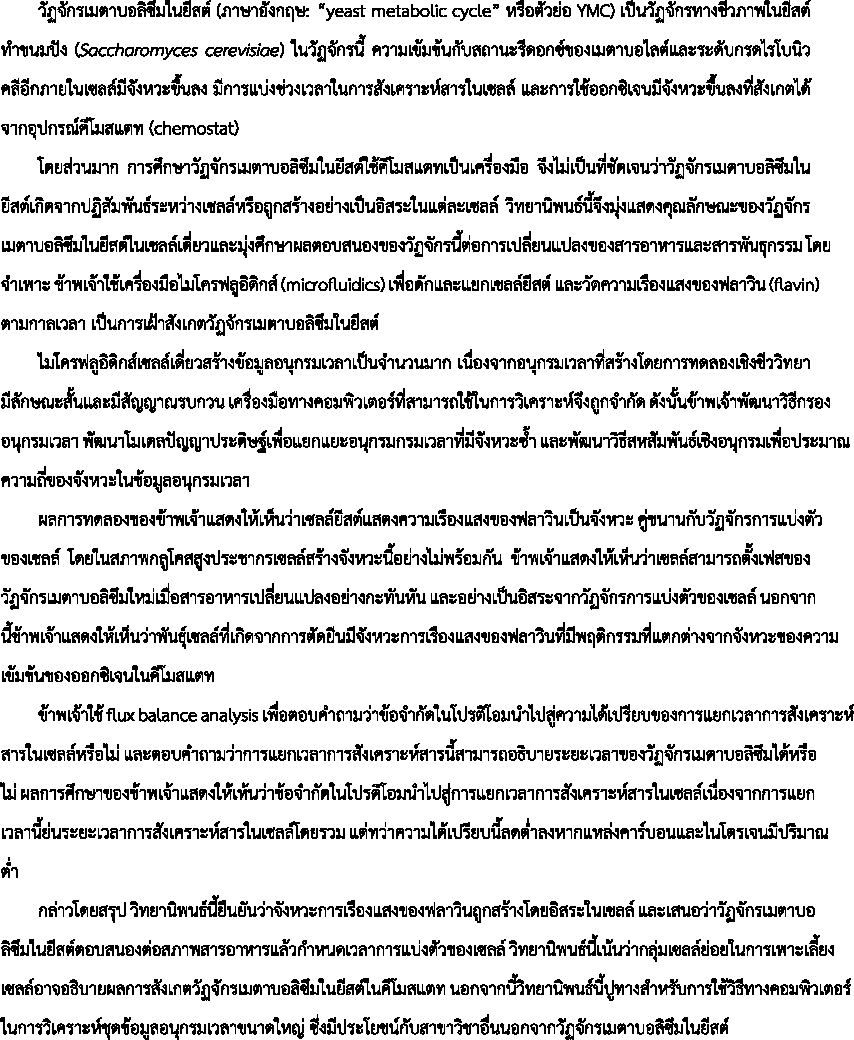
\includegraphics[width=\linewidth]{th_abstract_crop.pdf}
}

%%%% ACKNOWLEDGEMENTS

\acknowledgements{%
  This work would not have been possible without the support of many people and organisations.

  I would like to thank the financial support provided by School of Biological Sciences, University of Edinburgh, and the Edinburgh Global Scholarship.

  I would like to express my deepest gratitude towards my supervisors Dr Diego Oyarz\'{u}n and Prof Peter Swain for the unique opportunity of joining two research teams, and for creating such a great environment for me to learn and work in Edinburgh.
  I am also very grateful your advice, patience, and mental support --- especially in the very isolating days of the COVID-19 pandemic.

  I am most grateful for Dr Kevin Correia for his mentorship in the early parts of my PhD\@: especially teaching me how to me ask questions, bringing in laboratory best practices from his experience, and even philosophical insights in science and life.

  I am very grateful for the main software developers of the Swain lab: Dr Julian Pietsch, Dr Ivan Clark, Dr Diane Adjavon, and Dr Al\'{a}n Mu\~{n}oz Gonzalez.
  I would like to thank Julian in particular for his patience as I grasped the ropes of the old software pipeline.
  Thank you, Diane and Al\'{a}n, for including me in your very ambitious project to re-write the pipeline --- this was an immense learning experience for me.
  Al\'{a}n --- we've been through thick and thin, and I'm most grateful to have you as a partner in crime (?), and for \texttt{doom emacs} too.

  I am very grateful for Dr Ivan Clark and Iseabail Farquhar for imparting their wet-lab expertise and their patience during my experiments.
  Ish, I'd like to thank you for your patience and perseverance training me CRISPR during the chaotic times of the COVID-19 lockdown.

  I would also like to thank my other colleagues at the Swain Lab: Dr Fran\c{c}ois El-Daher, Dr Julien Hurbain, Dr Nahuel Manzanaro Moreno, Dr Yu Huo, and Sof\'{i}a Esteban Serna.

  I would like to thank my colleagues at the Biomolecular Control Group for creating a fantastic social environment and continuously sparking ideas.
  I am grateful for Dr Vanessa Smer-Barreto and Dr Babita Verma for their mentorship and feedback on my research.
  I would like to thank Dr Mona Tonn and Denise Thiel for our weekly movie nights and continued moral support.
  And I would like to thank Evangelos Marios-Nikolados for a great collaboration opportunity, and (too) regular pub nights.
  Let's drink to health!

  I would like to thank my friends from university --- Christos Nicolaou, Esther Ng, Patawee Jintana, among others --- for their moral support.
  I would like to extend special thanks to my best friends Jessica Wang and Maetavee Asavabhokhin for their unwavering emotional and moral support during all ups and downs.
  And I would also like to thank my high school friends, scattered across the globe, Attawit Chaiyaroj, Paloch Vasudhara, and Dr Pravarit Athiprayoon for their support too.

  Last but not least, I would like to thank my family.
  I express my deepest gratitude for my parents who have taught me the wonder of science, the importance of education, and the value of working hard.
  None of this would have been possible without you.
  Aunt Pinnapa, I now have a PhD\@!
  And lastly, I thank my brother Arun Wongprommoon and cousin Pornsom Ruengpirasiri for their continuous support in this long journey.
}

%%%% DECLARATION

%% Use a custom declaration

% \declaration{I did it.}

%% Use the standard regulation declaration. Enter your
%% name for the signature line.

\standarddeclaration{Arin Wongprommoon}

%%% Local Variables:
%%% mode: latex
%%% TeX-master: "../thesis"
%%% End:
